\documentclass[a4paper,10pt]{article}
\usepackage[utf8]{inputenc}
\usepackage{graphicx}
\usepackage{float}
\usepackage{caption}
\usepackage{subcaption}

%opening
\title{Machine Learning Final Report}
\author{Peter Ballen and Stephen Phillips}

\begin{document}
\maketitle

\section{Prinicpal Component Regression}
\subsubsection*{Semi-supervised Dimentionality Reduction}
Using Principal Component Regression. Using this technique alone actually got us past the first baseline. We used the MATLAB function svds to be able to compute it in a reasonable amount of time. For the first baseline we used 500 components. Then we run MATLAB's built in LASSO on the result.

Choosing the number of Pricipal Components was not arbitrary. We checked to see at what point the Pricipal Components gave diminishing returns. As it turns out the error keeps decreasing significantly as you add principal components for quite a while. We used 500 because it was computationally feasible and for memory reasons.

We analyzed the principal components to see what structure the data had. So we projected the data onto the princpal components and looked at the points and their score in the projected plane, as below.

\begin{figure}[H]
 \centering
 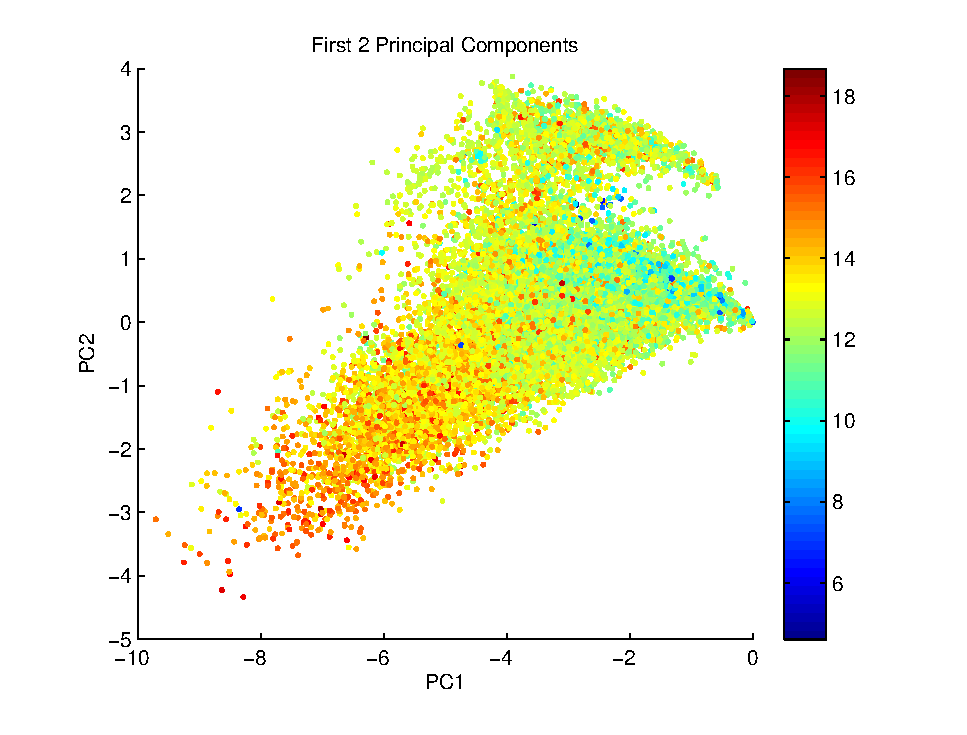
\includegraphics[scale=0.5]{First2PCs.eps}
 \caption{The first two pricipal components. The color represents the price (shown by the colorbar on the side)}
\end{figure}

As it turns out using the principal components on the words and bigrams and then running LASSO on the city labels and the PCA data is much better than working with the PCA data alone. We went from 0.86 RMSE to 0.81 RMSE on the testing set.

\begin{figure}[H]
 \centering
 \begin{minipage}{.5\textwidth}
    \centering
    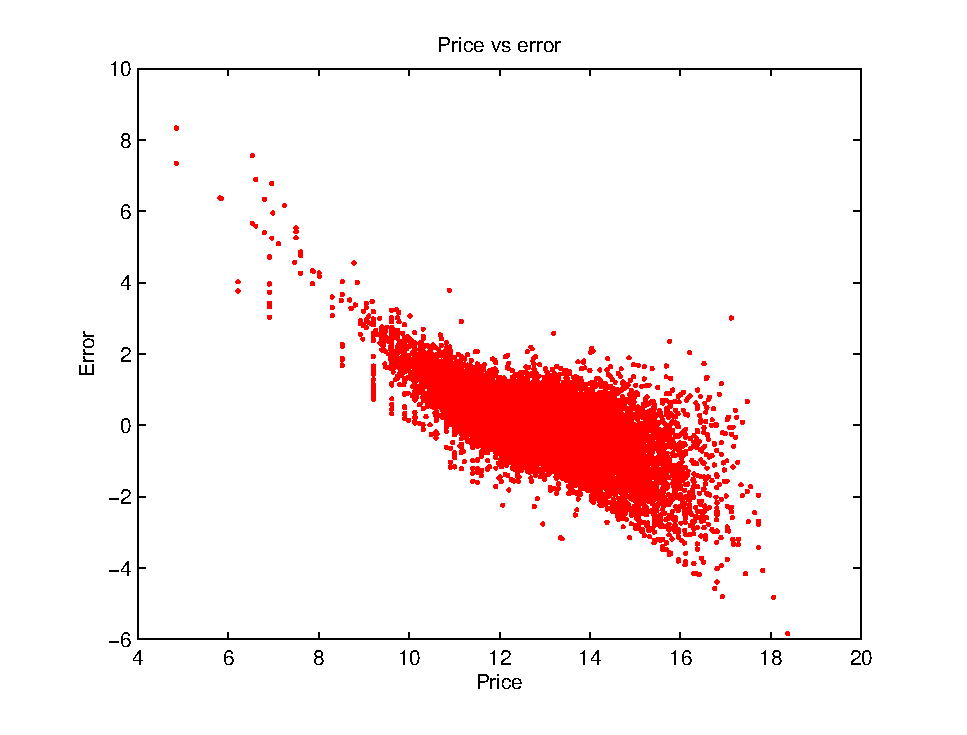
\includegraphics[width=6.0cm]{PCRPriceVsError.eps}
    \label{fig:fig1}
  \end{minipage}%
  \begin{minipage}{.5\textwidth}
    \centering
    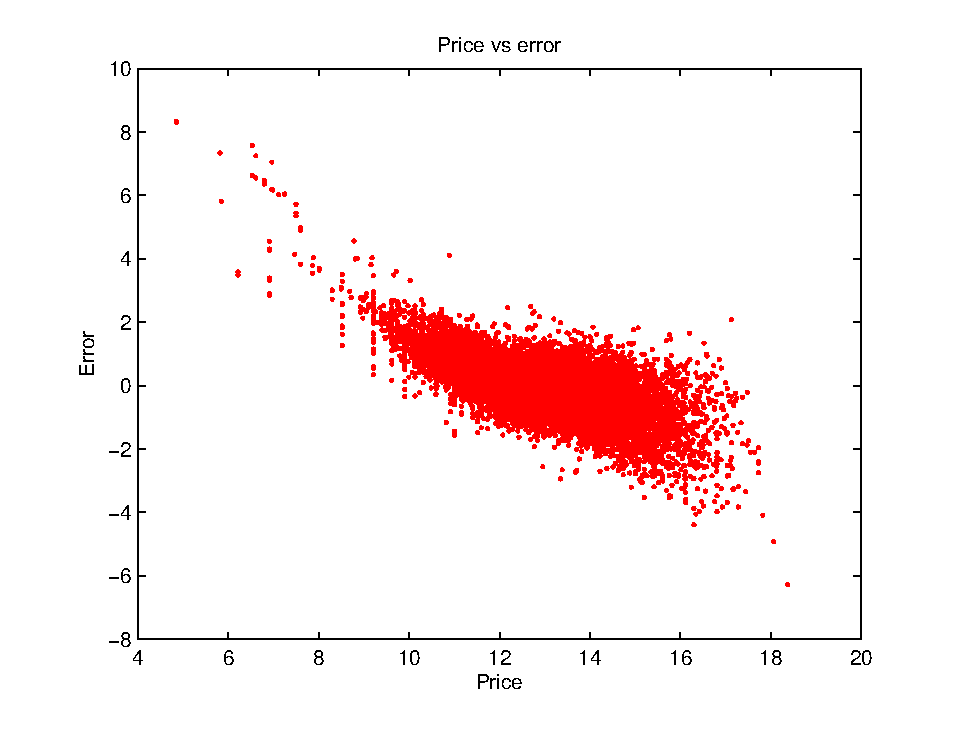
\includegraphics[width=6.0cm]{PCRPriceVsErrorWithCities.eps}
    \label{fig:fig2}
  \end{minipage}
 \caption{The errors of the PCR without cities (left) and with cities (right).
	  With the cities the curves on the edges are less pronounced}
\end{figure}


\section{Linear Regression with $L_1$ Regularization (LASSO)}
\subsection*{Simple Linear regression}
So instead of using the PCA data we used the full original dataset. As it turns out this performs quite well giving a RMSE of 0.75. Presumably using the full data gives more information and will the right regularization you can perform better than using the PCA data. We used this in our ensemble method (shown later) and it was one of the better drivers of performance.

\section{Linear Regression with $L_1$ Regularization and Hand Crafted Features}
\subsection*{Simple Linear regression}
To help improve things we also tried to add more features in to see if they would improve results. So we used feature interactions of the first 21 features (i.e. all products between them) which improved performance a bit getting the RMSE to 0.78. We also tried adding in a subset of the words (around 300 of them), feature selected using LASSO on the words and finding the highest weighted words. We also did this with the bigrams (adding less of them, about 200). Adding both of these improved the error to 0.76 RMSE. So creating features did help. Note that these improvements only happened after choosing the optimal lambda (which varied depending on the number of features intuitively). 


\section{SVM to separate data}
\subsubsection*{Discriminative Method}
Once again we use the PCA data. Then we train an SVM to spit the data with the small houses to everything else, the ones with Y above the 10th percentile and the others with Y below the it. We use MATLAB's built in svm classifier to do this. Then we train regressions (LASSO) on each half of that training data. Then we use the SVM to predict which half each point of the testing data should be on and predict with the appropriate weights. This did improve results over simply using the PCA data. The problem was the space was complicated enough that the number of support vectors was too large to fit under the 50MB limit. So while it improved the RMSE to 0.77 it ended up not being practical.


\section{Kernel Regression}
\subsubsection*{Instance Based Method}
We also ran Kernel regression using 11000 points (on the PCA data). We manage to get a RMSE of 0.73 using this. This method performed the best, and beat the second baseline. However, the method took to long to use as our final method. Generating 11000 distances for each of the 20000 test points was not fast enough unless you did it in batch. This performed the best most likely because it took into account the extremely pricing space the best. We expect that if we did kernel regression on the whole training set our RMSE would improve by a lot. We could not perform the kernel regression on more points because our computers kept running out of memory creating the n by n matrix of pairwise distances. So even training it took too much resources for us. This is why we tried reducing the dimentionality of the space using k-means (next section).

\section{K-Means as centers of Radial Basis Functions for Kernel Regression}
\subsubsection*{Generative Method/Instance Based Method}
We also tried using k-means on the PCA data with 2000 clusters (giving hopefully 100 points per cluster) and use the mean of the points in the cluster as the value of the center. As it turns out it is not nearly as good to use the cluster means as it is to use the whole dataset for kernel regression. The means are not too representative of the points as a whole. Perhaps if we had overclustered even more we may have gotten better results, however that ended up taking too long to compute. We also tried clustering on the word data directly, but this crashed MATLAB when we tried (after a long period of computation).

When looking at the range of clusters, we saw that there were many that were nearly empty and then several that had on the order of 200 points. The problem is that the way the data is distrubted there are places where many points are very close together even though their prices work very differently (Example shown below). This is why using kernel regression on the whole dataset works much better because it can account for these bad spots, whereas the means alone cannot.

\begin{figure}[H]
 \centering
 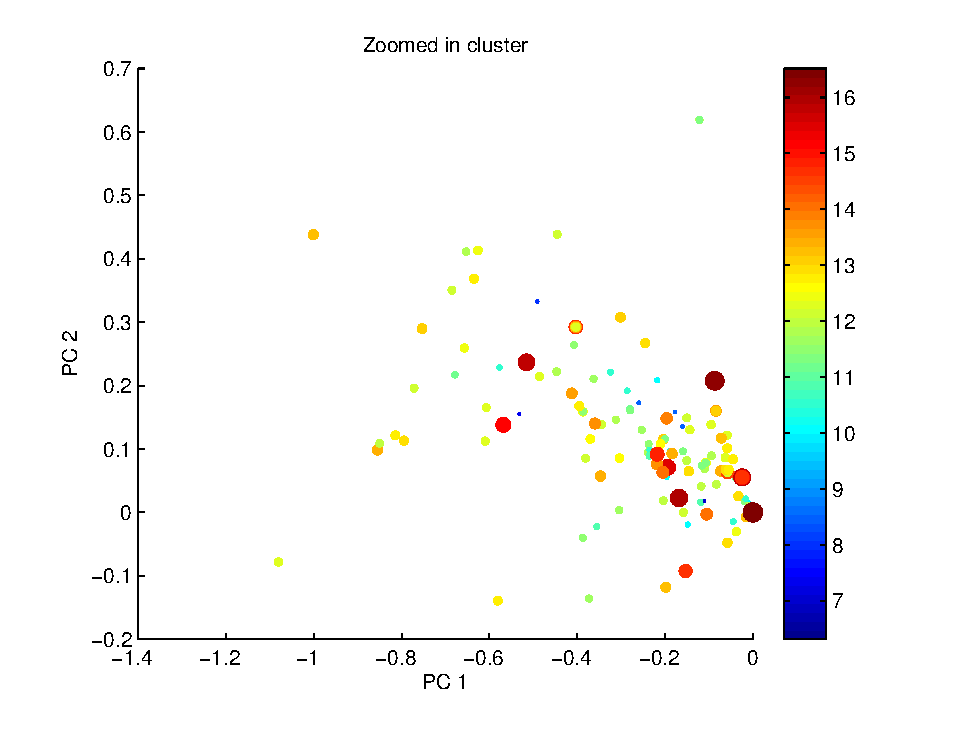
\includegraphics[scale=0.5]{ZoomedInCluster.eps}
 \caption{One of the larger clusters in our kmeans, zoomed in. Color and size show the price value of each point. As you can see, there are a large range of them all in very
	  close proximity, so using the mean of this cluster is not very informative.}
\end{figure}

\section{Ensemble}
\subsubsection*{Putting it all together}
The final submission we used was an ensemble method which ended up being the best. We trained on about 75 percent of the data chose the weights with the rest of the data then used those weightings of the different methods on the testing set. We get 0.75 RMSE which is our best method yet. We might have been able to play around with how we split the data to get better results, but we thought that this split was fairly good.

The results can be summarized in the table below
\begin{center}

\begin{tabular}{|c | c|}
\hline
 Technique & RMSE \\ \hline
Lasso with 500 PCs from word/bigram & 0.86457 \\ \hline
Lasso with 500 PCs plus city data & 0.8135 \\ \hline
Lasso with all 5007 features & 0.75695 \\ \hline
Lasso with hand-crafted features & 0.7632 \\ \hline
Lasso with SVM to identify cheap houses & 0.7754 \\ \hline
Kernel with 11000 points & 0.7352 \\ \hline
Kernel with 2000 mean points & 0.94641 \\ \hline
Clustering with Kmeans and Kernel Regression & 1.2169\\ \hline
Ensemble & 0.7545 \\ \hline

\end{tabular}
 
\end{center}


\end{document}
